\chapter{How to Rewrite Genes}

\begin{kaichang}
Leave the laboratory equipment alone for now and fetch a cup of yogurt from the kitchen.

Bacteria make yogurt: lactic-acid bacteria turn milk's lactose into lactic acid, making it sour and thick. A dairy's most dreaded accident is neither a power failure nor a milk shortage but an invader hundreds of times smaller than bacteria: a bacteriophage, a virus that infects them. Once inside a fermentation tank, it can wipe out the hardworking bacteria within hours. Milk stays milk instead of becoming yogurt, costing a large factory tons of product in one day.

Yet dairy engineers noticed something strange long ago: after certain phages attacked some bacterial strains once, the strains seemed to remember a grudge and no longer feared those viruses. Bacteria lack brains, nerves, and memory cells. How do they remember?

Unexpectedly, solving this puzzle gave humans a tool for rewriting almost any organism's genome. You have probably heard its name: CRISPR. We will travel from bacterial memory to human gene editing, then beyond the headlines to ask how reliable these scissors really are.
\end{kaichang}

\section{From Reading to Writing: Three Requirements}

Chapter 81 explained reading DNA's long book letter by letter. Reading requires eyes and patience; \textbf{editing} requires three things:

\begin{itemize}[itemsep=2pt]
\item \textbf{Find the page}: locate the intended site among billions of letters.
\item \textbf{Make the change}: delete, replace, or insert letters.
\item \textbf{Read it again}: verify the change and check for damage elsewhere.
\end{itemize}

Each is an independent technical hurdle. Historically, we learned fixed-pattern cutting and pasting before programmable cutting, and both tool generations came from bacteria.

Decades before CRISPR, scientists discovered bacterial antiviral weapons called \textbf{restriction endonucleases}. When phages inject DNA, these enzymes cut particular letter combinations. One enzyme, for instance, always recognizes GAATTC and cuts there, fragmenting the viral book and defeating invasion. Why spare bacterial DNA containing the same sequence? Bacteria attach chemical protective tags, methylation marks like those in Chapter 74, preventing recognition.

In the 1970s, scientists realized that fixed-sequence recognition makes these enzymes \textbf{molecular scissors that recognize letters}. Add molecular glue, \textbf{ligase}, to reconnect DNA ends. An energy note: joining ends forms phosphodiester bonds. Chapter 27's rule says bond formation releases energy, yet the overall ligase reaction still consumes ATP to drive it (Chapter 50). The old rules of energy-consuming bond breaking and energy-releasing bond making remain intact.

Scissors and glue supplied the first DNA cut-and-paste technology, \textbf{recombinant DNA}: remove a gene from one organism and join it to another DNA molecule. But each restriction enzyme recognizes only a fixed four- to eight-letter pattern; you cannot freely specify the cut site. For years, genetic rewriting therefore resembled \textbf{stamping parts with fixed dies}, not \textbf{writing on paper with a pen}.

\section{Plasmids and Transformation: Bacterial Copyists}

Cut-and-joined DNA needs a carrier to enter cells and be copied extensively. A \textbf{plasmid} is a small circular bacterial DNA molecule, only a few thousand letters, replicating independently of the main chromosome like a freely copied supplementary booklet.

The procedure cuts a plasmid with restriction enzymes, joins in the target gene using ligase, and returns it to bacteria. This last step, \textbf{transformation}, uses temperature changes, brief electrical pulses, or chemical treatment to create temporary openings in the membrane, Chapter 51's phospholipid boundary, through which plasmids enter. Each subsequent bacterial division copies the plasmid too. If it carries a protein recipe, bacteria can manufacture the protein, becoming living photocopiers and factories.

Transformation is inefficient: only a small fraction of cells acquire plasmids. To identify them, engineers preinstall an \textbf{antibiotic-resistance gene} as a ticket. On antibiotic-containing medium, cells without plasmids die; surviving colonies have received the cargo. This is Chapter 76's natural-selection logic---variation, selective pressure, and differential survival---with humans supplying the pressure.

\textbf{Translator safety note:} These cloning, transformation, and antibiotic-selection descriptions explain laboratory methods; they are not home protocols. Do not culture unknown microbes or generate and release resistant bacteria. Practical work requires an approved teaching or research setting with trained supervision and risk assessment. See \href{https://institute.acs.org/acs-center/lab-safety/education-training/safer-experiments.html}{ACS laboratory-safety guidance}.

\begin{qiaoliang}
Can bacterial copying turn invisible molecules into visible quantities? Suppose a common plasmid occurs at about 500 copies per bacterium, a culture reaches $10^{9}$ bacteria per milliliter, and we take one liter, or $10^{3}$ milliliters. The plasmid count is approximately
\[500 \times 10^{9} \times 10^{3} = 5\times 10^{14}\ \text{molecules}.\]
Using Chapter 5's Avogadro constant, $\ud{6.02\times 10^{23}}{mol^{-1}}$, this is roughly $10^{-9}$ moles, seemingly negligible. But a 5,000-base-pair plasmid has a molar mass around $\ud{3\times 10^{6}}{g\,mol^{-1}}$, yielding \textbf{a few milligrams} of DNA, enough to weigh and see in an electrophoresis gel (Chapter 81). One bacterium needs a microscope to be seen; a billion bacteria and their plasmids turn a molecular enterprise into milligrams of product. This underlies industries such as recombinant insulin, discussed in Chapter 83.
\end{qiaoliang}

\section{The Bacterial Archive: CRISPR's Original Job}

Return to the dairy puzzle. Bacterial memory occupies a peculiar genomic region: a long \textbf{repeat--spacer--repeat--spacer} pattern resembling a brick wall. Identical bricks, repeats of twenty or thirty letters, alternate with differing mortar joints, spacers. Its long name is clustered regularly interspaced short palindromic repeats: CRISPR.

Comparing spacer letters with viral genes produced a startling answer: \textbf{every mortar joint was a short viral DNA fragment}. When ancestral bacteria encountered phages, they clipped a small enemy photograph and inserted it into the archive, called \textbf{acquisition}. On renewed attack, they transcribed spacers into short RNAs, \textbf{wanted posters}, and handed them to Cas proteins such as Cas9. Carrying these posters, Cas proteins patrol the cell. When RNA pairs with matching viral DNA, Cas9 cuts the viral genome in two, called \textbf{interference}.

The molecular logic follows Chapter 66's double helix and Chapter 68's transcription: \textbf{targeting relies on complementary base pairing}. A pairs with T, or U in RNA, and G with C, recognizing letters through hydrogen bonding and geometry, not magic. Cas9 itself does not read the letters; the roughly twenty-letter guide RNA does.

Engineers made \textbf{one substitution}: replace the bacterial wanted poster with twenty letters of our own design. Cas9 becomes \textbf{programmable molecular scissors}. One vital detail remains: a short PAM sequence must lie beside the cut site, NGG for the most common Cas9, like a required parking space. Without it, the scissors refuse to act. This reduces accidental damage, but only reduces it, as we will see.

\section{After the Cut: Repair Determines the Outcome}

Headlines often stop at CRISPR cutting a gene, but cutting is only the start. Rewriting occurs when the cell \textbf{repairs the break}. A double-strand break is an emergency, and cells have two main repair teams whose consequences appeared in Chapters 67 and 72:

\begin{itemize}[itemsep=2pt]
\item \textbf{Direct end joining}, formally nonhomologous end joining, grabs and reconnects the ends. It is quick but rough, often losing or adding a few letters. A changed letter count shifts the subsequent reading frame (Chapter 69), scrambling protein instructions and \textbf{knocking out} the gene. One cut followed by imperfect cellular repair therefore has a good chance of disabling the target.
\item \textbf{Template-guided repair}, formally homology-directed repair, uses nearby DNA homologous to both sides as a template for accurate restoration. Supply a designed template, and the cell can replace particular letters or insert a whole new gene, called \textbf{knock-in}. Unfortunately, this precise pathway is inefficient in most cells and mainly active during cell division, one reason accurate rewriting remains difficult.
\end{itemize}

\begin{center}
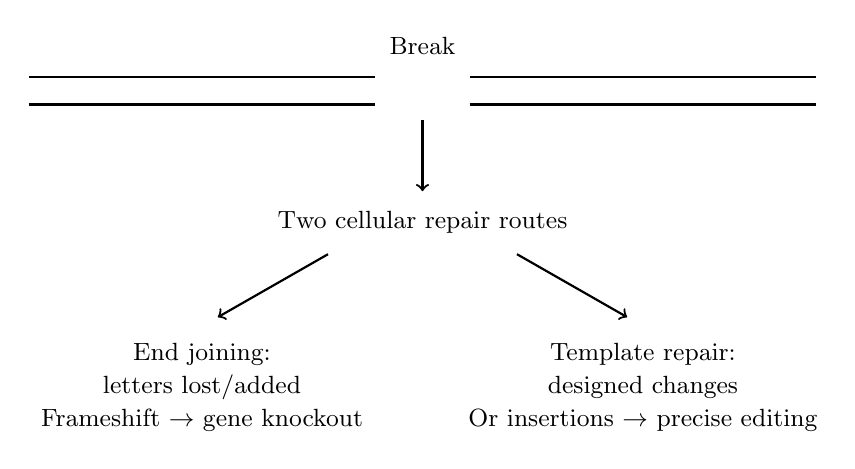
\begin{tikzpicture}
\draw[thick] (0,0) -- (4.4,0);
\draw[thick] (5.6,0) -- (10,0);
\draw[thick] (0,0.35) -- (4.4,0.35);
\draw[thick] (5.6,0.35) -- (10,0.35);
\node at (5,0.75) {\small Break};
\draw[->,thick] (5,-0.2) -- (5,-1.1);
\node at (5,-1.5) {\small Two cellular repair routes};
\draw[->,thick] (3.8,-1.9) -- (2.4,-2.7);
\node[align=center,anchor=north] at (2.2,-2.9) {\small End joining:\\ \small letters lost/added\\ \small Frameshift $\rightarrow$ gene knockout};
\draw[->,thick] (6.2,-1.9) -- (7.6,-2.7);
\node[align=center,anchor=north] at (7.8,-2.9) {\small Template repair:\\ \small designed changes\\ \small Or insertions $\rightarrow$ precise editing};
\end{tikzpicture}
\end{center}

The diagram is a representation: two horizontal lines stand for double-stranded DNA and arrows for cellular choices. Real repair involves several proteins working at nanometer scales, with no signposted fork. Which route a break takes depends on cell type, cell-cycle stage, and chance, explaining why one editing experiment yields different outcomes in different cells.

\begin{zhengju}
This tool did not appear from a lone genius's imagination. Its story began with ``We do not know what this is.''

In 1987, Yoshizumi Ishino's Japanese team studying an E. coli gene noticed nearby repeats: short passages reading the same forward and backward, separated by diverse fragments. Unable to explain them, they honestly reported that their biological significance was unknown. Scientific honesty often begins with an unassuming sentence.

In the 1990s, Spanish microbiologist Mojica encountered similar structures in extremely salt-loving archaea. Following them for more than a decade, he found widespread bacterial and archaeal repeats with ever-changing spacers. In 2003, he suggested antiviral defense. In 2005, three teams independently compared spacers with databases and found many \textbf{exact phage-DNA matches}, establishing the hypothesis of a bacterial acquired-immunity archive. Alternatives remained: coincidence or other regulatory functions. The hypothesis needed an experiment distinguishing explanations, not more agreement.

The key experiment came in 2007 from an unexpected setting: a laboratory of Danish dairy-ingredient company Danisco, not a famous university. Barrangou, Horvath, and colleagues exposed yogurt-making Streptococcus thermophilus to phages and examined survivors. Their CRISPR regions gained new spacers exactly matching the attacker. Deleting a spacer removed its corresponding resistance; introducing one provided previously absent resistance. Manipulating one variable produced the corresponding causal effect, firmly supporting the archive hypothesis.

The final mechanistic piece arrived in 2012: Charpentier and Doudna's team purified Cas9 and two RNAs, reassembled them in vitro, and showed that one designed guide RNA could direct cutting at any chosen DNA site. Programmability was directly demonstrated in a flask. In 2013, Feng Zhang's and Church's teams almost simultaneously adapted the system to human and mouse cells, editing mammalian genomes. Charpentier and Doudna received the 2020 Chemistry Nobel Prize.

Twenty-five years led from unexplained repeats to rewriting life: recording anomalies, comparing databases, proposing hypotheses, performing interventions, and reconstructing mechanisms in tubes. Remember not who was cleverest but that every link in the evidence chain could have been overturned.
\end{zhengju}

\section{Where the Scissors Go Wrong}

Now for what headlines omit. Genetic scissors are such an effective metaphor that they mislead: scissors suggest clean, precise, on-demand cuts. Real editing faces at least three formidable hurdles.

\textbf{First: off-target editing.} Twenty-letter guide recognition is probabilistic, not black and white. Among three billion human letters, a passage differing by only one or two letters may still pair sufficiently for Cas9 to cut unintentionally. Consequences vary: an unimportant region may tolerate it, while another gene may acquire a harmful mutation, sometimes activating cancer-related pathways (Chapter 80). Improved Cas proteins and guides reduce off-target rates, but low is not zero.

\textbf{Second: mosaicism.} Even perfect targeting does not edit every cell simultaneously. Of thousands or millions of cells, some edit successfully, others remain unchanged, and others acquire differing outcomes. The tissue or embryo becomes a patchwork with different sequences in its patches, called mosaicism. Early embryonic editing particularly often produces this because several cells may exist by the time editing finishes, with only some carrying the desired change. An edited embryo may thus mean only a partly edited embryo.

\textbf{Third: delivery.} This unromantic hurdle is often hardest: even excellent scissors must \textbf{reach the right cells}. Outside the body, cells can be removed, editing tools introduced electrically, and edited cells returned, as in some therapies discussed in Chapter 83. Direct editing inside the body requires couriers for Cas9 and guide RNA, commonly disarmed viral vectors or lipid nanoparticles, using the lipid and membrane chemistry of Chapters 47 and 51. The blood-rich liver is relatively accessible; the brain's blood--brain barrier makes delivery difficult. Packaging itself can alert immunity (Chapter 61), causing failure or injury. Delivery often separates success in a tube from success in a patient.

\textbf{Translator safety note:} Genome editing and delivery are not self-treatment procedures. Do not use DIY gene-therapy kits or administer editing materials to yourself or anyone else. Any proposed treatment needs qualified clinical care and appropriate regulatory oversight. See \href{https://www.fda.gov/vaccines-blood-biologics/cellular-gene-therapy-products/information-about-self-administration-gene-therapy}{FDA's self-administration warning}.

\begin{wuqu}
``CRISPR is like find-and-replace in a word processor: enter the sequence and get a precise correction.''

The analogy fails three ways. Find-and-replace \textbf{does not misspell}, whereas guides tolerate mismatches and may edit similar passages. It \textbf{does not edit only half the document}, whereas mosaics contain edited and unedited cells. And a document \textbf{needs no courier}, whereas bodily targets require delivery by vectors or lipid particles. A better image sends a courier who recognizes twenty letters, occasionally misreads one or two, into a three-billion-letter library continually copying and repairing itself. Editing success, accuracy, and delivery are three independent examinations, any of which can be failed. Calling CRISPR error-free scissors conceals all three.
\end{wuqu}

\begin{tiaozhan}
Why can twenty letters still identify the wrong target? Using Chapter 81's combinatorial intuition, a specific twenty-letter sequence appears randomly with probability $4^{-20}\approx 10^{-12}$. Across $3\times 10^{9}$ genomic letters, accidental exact matches seem almost impossible, explaining why twenty letters can locate a target. Off-target cutting involves \textbf{approximate matches}: one mismatch has $20\times 3=60$ possibilities, and two have $\binom{20}{2}\times 3^2\approx 1700$. Scatter thousands of near-matches across three billion letters, and a few resemblances become an expected statistical outcome rather than a bizarre accident. Engineers therefore work hard to make Cas recognition stricter: they are fighting combinatorics, not isolated mishaps. You can skip this derivation, but it helps you judge reported reductions in off-target rates.
\end{tiaozhan}

\section{Finer Tools: Base and Prime Editing}

Breaking both strands and gambling on repair is crude. Can one letter change \textbf{without a double-strand break}? \textbf{Base editing}, introduced from 2016 onward, does this. Engineers blunt Cas9's cutting edge so guides still position it but it no longer breaks both strands, then attach an enzyme that changes C to T or A to G. Many inherited diseases arise from \textbf{one letter}; for these, base editing resembles a pencil and eraser, gentler than scissors, with large break-induced insertions and deletions almost disappearing. Its clear limitation is a restricted conversion menu: if the needed change is absent, it cannot help.

\textbf{Prime editing}, introduced in 2019, goes further. Cas9 nicks one strand and carries reverse transcriptase; an extended guide RNA includes a small template for new text. At the target, the machine \textbf{copies} those letters into the genome. CRISPR plus a template cuts a page and hopes a copyist follows the supplied sample; prime editing opens the page and traces over the error on site. In principle it permits any base substitution and small insertions or deletions. Yet it is young: efficiency remains limited, delivery difficult, and errors possible. It lowers the three hurdles rather than removing them.

\begin{table}[htbp]
\centering
\caption{Generations of gene-editing tools; the comparisons are memory aids, not literal descriptions}
\begin{tabular}{llll}
\toprule
Tool & Resembles & Strength & Main limitation \\
\midrule
\shortstack[l]{Restriction enzyme\\plus ligase} & \shortstack[l]{Fixed die\\plus glue} & \shortstack[l]{Joining and\\cloning DNA} & Fixed cutting sites \\
\shortstack[l]{CRISPR\\knockout} & \shortstack[l]{Programmable\\scissors} & \shortstack[l]{Disabling a\\target gene} & \shortstack[l]{Off-target cuts;\\variable repair} \\
\shortstack[l]{CRISPR\\plus template} & \shortstack[l]{Scissors\\plus copyist} & \shortstack[l]{Precise substitutions\\and insertions} & \shortstack[l]{Low efficiency;\\needs dividing cells} \\
Base editing & \shortstack[l]{Pencil\\and eraser} & \shortstack[l]{Single-letter\\conversions} & \shortstack[l]{Only certain\\conversions} \\
Prime editing & \shortstack[l]{Search\\and replace} & \shortstack[l]{Arbitrary changes\\over small regions} & \shortstack[l]{Efficiency and\\delivery limits} \\
\bottomrule
\end{tabular}
\end{table}

The direction is clear: targeting becomes more flexible, interventions gentler, and less is left to cellular improvisation. Yet every limitations column still contains unfinished business.

\section{Where the Tools Have Limits}

Every tool has boundaries, and gene editing especially requires candid warnings.

First, it works best for \textbf{single-gene problems with clear causality}: one letter, one gene, one disease, and a clear target. Height and most common-disease risks instead combine hundreds or thousands of small genetic effects with environment (Chapters 73 and 85). There is no single cut to make or obvious target waiting anywhere in the genome.

Second, even with a clear target, \textbf{somatic editing} differs from \textbf{germline editing}. Changes in a patient's marrow or liver end with that person; changes in embryos or reproductive cells enter every future generation. The former treats disease, the latter decides for unborn people who cannot consent. Drawing the boundary is ethical as well as technical, as Chapter 83 discusses.

Third, rewriting letters does not mean understanding their \textbf{rules of use}. Chapter 70 compared genes with dimmable rather than permanently lit lamps; Chapter 74 showed altered usage without sequence change. Correcting a letter still leaves its effects in liver versus brain, at ten versus fifty years old, in another partly unread book.

\begin{shiyan}
\textbf{Invite DNA Out of Fruit} (for classroom or home; no genes are edited, only extracted for observation).

Materials: half a ripe banana or two strawberries, a teaspoon of salt, two drops of dish detergent, half a cup of warm water, gauze or coffee-filter paper, a clear cup, and a cup of medical alcohol refrigerated for half an hour.

Procedure: (1) Put fruit, warm water, salt, and detergent in a food-storage bag and mash for two or three minutes. Salt encourages DNA aggregation, and detergent disrupts cell and nuclear membrane phospholipids (Chapter 51). (2) Filter through gauze into the cup. (3) Slowly pour cold alcohol down the cup wall to form a separate layer without stirring. (4) Wait five minutes and watch the interface.

What to observe: white clumps or threads gradually appear between the layers and can be wound around a chopstick. They are tangled DNA released by hundreds of millions of banana cells.

Safety reminder: alcohol is \textbf{flammable}; keep it away from flames and recap afterward. Detergent-contacted materials \textbf{must not be eaten}. Wash with soap afterward.

Think: these white clumps contain all banana genes. Yet locating, cutting, repairing, and delivering remain four hurdles between extraction and editing one gene. Handle DNA yourself, then reconsider how long that tool chain is.
\end{shiyan}

\textbf{Translator safety note:} Do not follow the household-refrigerator instruction for flammable alcohol. Ordinary refrigerators and freezers are not suitable for flammable chemical storage; have a qualified teacher choose a safe preparation method or prepared demonstration. Adults should handle alcohol with eye protection, away from heat, sparks, and flames. Use the chopstick to lift material, not bare hands, and never taste it. See \href{https://ehs.stanford.edu/wp-content/uploads/Lab-Compliance-Cheat-Sheet.pdf}{Stanford flammable-storage precautions}, \href{https://www.poison.org/articles/rubbing-alcohol-only-looks-like-water}{Poison Control alcohol guidance}, and \href{https://www.acs.org/education/celebrating-chemistry-editions/2024-ccew/science-safety-tips.html}{ACS activity safety}.

\section{Back to the Yogurt}

Why can lactic-acid bacteria remember? Their genomic archive stores a small piece of enemy DNA after each survived phage attack. Cas proteins patrol with RNA wanted posters transcribed from those fragments and cut returning enemies apart. This is genuine acquired immunity, arising billions of years before vertebrate antibodies and writing memory directly into inheritable DNA.

At the molecular level, humans did just one thing: \textbf{replace the wanted poster with our own}. Bacterial defense archives became editing tools. The dairy industry still uses the original mechanism too, examining CRISPR archives to breed fermentation strains resistant to circulating phages. Reliable yogurt production partly depends on this billions-of-years-old bacterial memory. From yogurt to a Nobel Prize, viral scraps to life's editing pencil, no step appeared from nowhere.

\section{After Editing, the Questions Begin}

Gene editing raises two larger sets of questions. Medical questions ask how tools become medicines: recombinant insulin, gene therapy, the boundary between somatic treatment and germline editing, and CAR-T cells removed, modified, and returned. These belong to Chapter 83. Ecological and social questions ask whether engineered organisms' genes can escape from fields into wild populations and who sets the boundaries of rewriting life; Chapter 84 follows those. You can already see what is truly scarce: not the ability to cut, but knowledge and safeguards governing \textbf{whether to cut, where, and what happens if it goes wrong}.

\section*{Try It Yourself}

\begin{sikaoti}
\item Draw the flow from a first phage attack to bacterial resistance. Mark where DNA, RNA, and proteins enter, and identify acquisition and interference.
\item Why does targeting need about twenty letters rather than four? Four-letter sequences have $4^4=256$ possibilities; how often would one occur on average in a three-billion-letter genome? What about twenty letters? (Use $4^{20}\approx 10^{12}$.)
\item Why does the same cut usually produce a knockout, while precise rewriting requires a template and good luck? Explain from the operating conditions of the two repair routes.
\item Someone claims a CRISPR-edited plant is absolutely safe. Design a verification approach to check the intended site and off-target changes. (Hint: combine these tools with Chapter 81's sequencing.)
\item Editing a four-cell embryo successfully changes only one cell. Roughly what fraction of the resulting individual's cells carry the edit? If germ cells are absent from that fraction, is it inherited? How should ``we edited an embryo'' be stated more precisely?
\item Restriction enzymes recognize fixed sequences such as GAATTC, also present in bacterial genomes. How do bacteria protect themselves? How does self-labeling resemble Chapter 61's immune distinction between self and invaders?
\end{sikaoti}
